\chapter{Consuming Linked Data}
\label{ch:ch5}

\begin{itemize}
\item Survey on visualizations for RDF
\item Contrib 1: Wizard for visualizations
\item Contrib 2: Vocabularies for describing visualizations
\item Contrib 4: Revealing the ``important'' properties of Entities for visualizations
\item Contrib 5: Focus on Event--Confomaton
\item Contrib 6: Focus on statistics -Concrete applications: PerfectSchool, French Amenities.
\item Contrib 7: Apps4Europe: Improving the discovery of application contests in Open Data Events

\end{itemize}


\section{A vocabulary for Describing VIsualization Applications} \label{sec:dvia}

We have implemented a vocabulary, DVIA\footnote{\url{http://bit.ly/Vb4L8k}} aims at describing any applications developed to consume datasets in 4-5 stars, using visual tools to showcase the benefits of Linked Data. It reuses four existing vocabularies: Dublin Core terms at \url{http://purl.org/dc/terms/}, dataset catalogue (DCAT) at \url{http://www.w3.org/ns/dcat#}, Dublin Core Metadata Initiative at \url{http://purl.org/dc/dcmitype} and the Organization vocabulary at \url{http://www.w3.org/ns/org#}.  It is composed of three main classes : 

\begin{itemize}
\item \textbf{Application}: This class represents the application or the mashup developed for demo-ing or consuming data in LD fashion. It is subclass of \textbf{dctype:Software}
\item \textbf{Platform}: The platform where to host or use the application, could be on the Web (Firefox, Chrome, IE, etc..) or mobile (android, iOS, mobile ) or even desktop
\item \textbf{VisualTool}: Represents the tool or library used to build the application. 
\end{itemize}

The diagram of the main classes and properties is depicted in Figure \ref{visuGraphModel}. The current version of the vocabulary in Turtle format can be found at \url{http://www.eurecom.fr/~atemezin/datalift/visumodel/visu-vocab.ttl} .  Listing \ref{snapshot} is a snapshot of the description of the application which won the Semantic Web Challenge\footnote{\url{http://challenge.semanticweb.org/2012/winners.html}} in 2012, the \textit{EventMedia Live} application, described using DVIA vocabulary. It depicts apart from some metadata about the application (dct:title, dct:name, dct:issued, dct:creator and dct:license), the different visualization libraries integrated for building Eventedia Live (e.g.: Google API, Backbone, etc), as well as the operating systems where it is designed for, the different views/facets available in the application (map, charts, graphs, force-directed layout, ect) and the heteregeneous datasets used to implement it. 
\lstset{basicstyle=\scriptsize, backgroundcolor=\color{white}, frame=single, caption= {Snapshot in Turtle of the description of Event Media Live Application}, label=snapshot, captionpos=b}
\begin{lstlisting}

visuapp:eventMedia01
       a dvia:Application ; 
       dct:title "EventMedia Live"@en;   
       dvia:description "An application for reconciling Live events with media" ; 
       dvia:url <http://eventmedia.eurecom.fr> ; 
       dct:issued "2012-11-10"^^xsd:date ; 
       dvia:businessValue "not commercial" ;   
       dvia:keyword "events, media"^^xsd:string ; 
       dct:license <http://www.opendatacommons.org/licenses/pddl/1.0/> ; 
      dvia:platform [ a dvia:Platform ; 
			dct:title: "Desktop" ;
			dvia:preferredNavigator "Google Chrome" ; 
			dvia:alternativeNavigator "FireFox" ;
			dvia:system "Mac OS, Windows, Linux"^^string ] ; 
		
     dvia:usesTool [ a dvia:visualTool; dct:title "Google visualization Tool" ; 
	dct:description "Google visualization API" ; 
	dvia:accessUrl <https://developers.google.com/chart/interactive/docs/reference> ; 
	dvia:downloadUrl <http://www.google.com/uds/modules/gviz/gviz-api.js/> ] ;
    dvia:usesTool visuapp:visualTool02 ;
    dvia:consumes [ a dcat:Dataset; dct:title "BBC dump"] ; 
    dvia:consumes [ a dcat:Dataset; dct:title "last.fm scrapped dataset"] ;
    dvia:consumes [ a dcat:Dataset; dct:title "upcoming scrapped dataset"] ;
    dvia:consumes [ a dcat:Dataset; dct:title "eventful scrapped dataset"] ;
    dvia:consumes [ a dcat:Dataset; dct:title "Flickr scrapped dataset"] ;
    dvia:consumes [ a dcat:Dataset; dct:title "Music Brainz "] ;
    dvia:consumes [ a dcat:Dataset; dct:title "Foursquare Json file"] ;
    dvia:consumes [ a dcat:Dataset; dct:title "DBpedia"] ;
    dct:creator [foaf:mbox "khrouf@eurecom.fr"; foaf:name "Houda Khrouf"];
    dct:creator [foaf:mbox "vuk@eurecom.fr"; foaf:name "Vuk Milicik"];
    dct:creator [foaf:mbox "raphael.troncy@eurecom.fr"; foaf:name "Raphael Troncy"];
    dvia:view "map, chart, graph, force-directed layout" ; 
       .
	   ...
	
\end{lstlisting}

The full version of this sample description is available at \url{http://www.eurecom.fr/~atemezin/datalift/visumodel/eventMedia-sample.ttl}. The actual version of the DVIA intends to be small enough to cover the concepts that are needed to reuse partial or full parts of applications. 

\begin{figure}[!htbp]
  \begin{center}
    %\leavevmode
      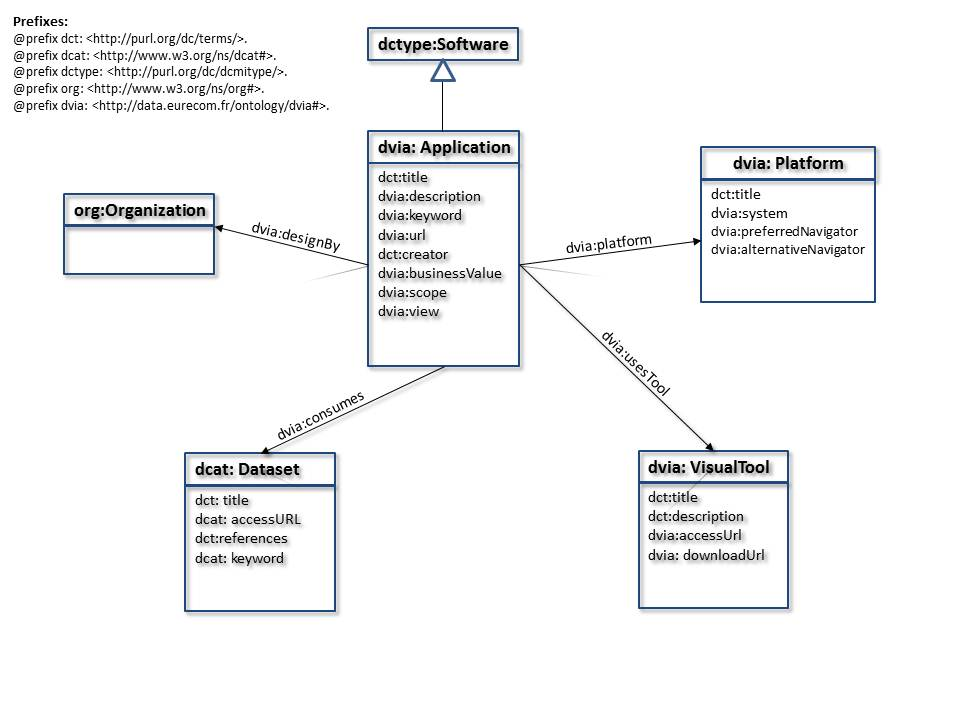
\includegraphics[ height=5in]{img/visuGraphModel.jpg}
  
    \caption{Conceptual Model of the DVIA vocabulary }
    \label{visuGraphModel}
  \end{center}
\end{figure}



\subsection*{Conclusion} \label{sec:conclusion}
% deploy the vocab and setting up a hub for mashups
% find patterns for applications
% develop a recommender for creating applications according to some criteria
\todo{Rewrite properly this section}
\textcolor{red}{We have presented in this paper an approach that could help reusing tools and libraries in the domain of applications built on top of datasets in Linked Open Data. We first presented our motivation as to demonstrate to the end users or decision makers, there is always a need to develop a showcase, hence sometimes looking for analogous or similar applications in the area to ease the process of creation the mashup. We proceeded by surveying some applications to extract relevant common facts worth reusable, from which we proposed a small vocabulary (DVIA)  to semantically describe visual applications. }

\textcolor{red}{We need to validate the DVIA by scrapping and reconciling data from all innovative applications websites and exposed them in RDF, starting with some of those we studied and others applications submitted at the Semantic Web Challenge the past three years. We strongly believe that having such a a hub  describing the tools, datasets, etc.  used to build  applications consuming 4-5 stars datasets will contribute to interoperable Applications leading to a Linked Open Visualizations (LOVIZ) on the LOD cloud.}


\section{Important Properties for an Entity}
\label{sec:propEntities}
In many knowledge bases, entities are described with numerous properties. However, not all properties have the same importance. Some properties are considered as keys for performing instance matching tasks while other properties are generally chosen for quickly providing a summary of the key facts attached to an entity. Our motivation is to provide a method enabling to select what properties should be used when depicting the summary of an entity, for example in a multimedia question answering system such as QakisMedia\footnote{\url{http://qakis.org/}} or in a second screen application providing more information about a particular TV program\footnote{\url{http://www.linkedtv.eu/demos/linkednews/}}. Our approach consists in: (i) reverse engineering the Google Knowledge Panel by extracting the properties that Google considers as sufficiently important to show (Section~\ref{sec:knowledge-graph}), and (ii) analyzing users' preferences by conducting a user survey and comparing the results (Section~\ref{sec:evaluation}). We finally show how we can explicitly represent this knowledge of preferred properties to attach to an entity using the Fresnel vocabulary\todo{TODO: ADD reference here?}

\subsection{Reverse Engineering the Google KG Panel}
\label{sec:knowledge-graph}
Web scraping is a technique for extracting data from Web pages. We aim at capturing the properties depicted in the Google Knowledge Panel (GKP) that are injected in search result pages~\cite{Bergman2012}. We have developed a Node.js application that queries all DBpedia concepts that have at least one instance which is \texttt{owl:sameAs} with a Freebase resource in order to increase the probability that the search engine result page (SERP) for this resource will contain a GKP. We assume in our experiments that the properties displayed for an entity are type and context dependent (country, time, query) which can affect the results. Moreover, we filter out generic concepts by excluding those who are direct subclasses of \texttt{owl:Thing} since they will trigger ambiguous queries. We obtained a list of $352$ concepts\footnote{See also the SPARQL query at \url{http://goo.gl/EYuGm1}}.

\begin{algorithm}[h]\scriptsize
\caption{Google Knowledge Panel reverse engineering algorithm} \label{algoscrapping}
\begin{algorithmic}[1]
    \STATE INITIALIZE $equivalentClasses(DBpedia,Freebase) $ AS $vectorClasses$
    \STATE Upload $vectorClasses$ for querying processing
    \STATE Set $n$ AS number-of-instances-to-query
    \FOR {each $conceptType \in vectorClasses$}
	\STATE SELECT $n$ instances
	\STATE $listInstances \leftarrow$ SELECT-SPARQL($conceptType$, $n$)
		\FOR {each $instance \in listInstances$}
			\STATE CALL http://www.google.com/search?q=$instance$
			\IF {$knowledgePanel$ exists}
				\STATE SCRAP GOOGLE KNOWLEDGE PANEL
			\ELSE
				\STATE CALL http://www.google.com/search?q=$instance + conceptType$
 				\STATE SCRAP GOOGLE KNOWLEDGE PANEL
			\ENDIF
			\STATE $gkpProperties \leftarrow$ GetData(DOM, EXIST(GKP))
			
		\ENDFOR
	\STATE COMPUTE occurrences for each $prop \in gkpProperties$
    \ENDFOR
    \RETURN $gkpProperties$
\end{algorithmic}
\end{algorithm}
\normalsize
For each of these concepts, we retrieve $n$ instances (in our experiment, $n$ was equal to 100 random instances). For each of these instances, we issue a search query to Google containing the instance label. Google does not serve the GKP for all user agents and we had to mimic a browser behavior by setting the $User-Agent$ to a particular browser. We use CSS selectors to check the existence of and to extract data from a GKP. An example of a query selector is $.\_om$ (all elements with class name $\_om$) which returns the property DOM element(s) for the concept described in the GKP. From our experiments, we found out that we do not always get a GKP in a SERP. If this happens, we try to disambiguate the instance by issuing a new query with the concept type attached. However, if no GKP was found again, we capture that for manual inspection later on. Listing~\ref{algoscrapping} gives the high level algorithm for extracting the GKP. The full implementation can be found at \url{https://github.com/ahmadassaf/KBE}. We finally observe that this experiment is only valid for the English Google.com search results since GKP varies according to top level names.


\subsection{Evaluation}
\label{sec:evaluation}
We conducted a user survey in order to compare what users think should be the important properties to display for a particular entity and what the GKP shows.

\paragraph{\textbf{User survey.}}
\label{sec:survey}
We set up a survey\footnote{The survey is at \url{http://eSurv.org?u=entityviz}} on February 25th, 2014 and for three weeks in order to collect the preferences of users in term of the properties they would like to be shown for a particular entity. We select only one representative entity for nine classes: \texttt{TennisPlayer}, \texttt{Museum}, \texttt{Politician}, \texttt{Company}, \texttt{Country}, \texttt{City}, \texttt{Film}, \texttt{SoccerClub} and \texttt{Book}. 152 participants have provided answers, 72\% from academia, 20\% coming from the industry and 8\% having not declared their affiliation. 94\% of the respondents have heard about the Semantic Web while 35\% were not familiar with specific visualization tools. The detailed results\footnote{\url{https://github.com/ahmadassaf/KBE/blob/master/results/agreement-gkp-users.xls}} show the ranking of the top properties for each entity. We only keep the properties having received at least 10\% votes for comparing with the properties depicted in a KGP. We observe that users do not seem to be interested in the \texttt{INSEE code} identifying a French city while they expect to see the \texttt{population} or the \texttt{points of interest} of this city.
\paragraph{\textbf{Comparison with the Knowledge Graphs.}}
\label{sec:comparison}
The results of the Google Knowledge Panel (GKP) extraction\footnote{\url{https://github.com/ahmadassaf/KBE/blob/master/results/survey.json}} clearly show a long tail distribution of the properties depicted by Google, with a top N properties (N being 4, 5 or 6 depending on the entity) counting for 98\% of the properties shown for this type. We compare those properties with the ones revealed by the user study. Table~\ref{tab:agreement} shows the agreement between the users and the choices made by Google in the GKP for the 9 classes. The highest agreement concerns the type \texttt{Museum} (66.97\%) while the lowest one is for the \texttt{TennisPlayer} (20\%) concept. We think properties for museums or books are more stable than for types such as person/agent which vary significantly. We acknowledge the fact that more than one instance should be tested in order to draw meaningful conclusion regarding what are the important properties for a type.
\begin{table}[!htp]
\centering{\scriptsize
\begin{tabular}{lccccccccc}
\hline
 \textbf{Classes}	& TennisPlayer 	& Museum & Politician & Company & Country & City & Film & SoccerClub & Book	 \\ \hline
 \textbf{Agr.}& 20\%  & 66.97\% & 50\% & 40\% & 60\% & 60\% & 60\% & 50\% & 60\% \\ \hline
\end{tabular}
\caption{Agreement on properties between users and the Knowledge Graph Panel}
\label{tab:agreement}
}
\end{table}\normalsize

With this set of 9 concepts, we are covering $301,189$ DBpedia entities that have an existence in Freebase, and for each of them, we can now empirically define the most important properties when there is an agreement between one of the biggest knowledge base (Google) and users preferences.

\paragraph{\textbf{Modeling the preferred properties with Fresnel.}}
\label{sec:fresnel}
Fresnel\footnote{\url{http://www.w3.org/2005/04/fresnel-info/}} is a presentation vocabulary for displaying RDF data. It specifies \textit{what} information contained in an RDF graph should be presented with the core concept \texttt{fresnel:Lens}~\cite{pietriga2006}. We use the Fresnel and PROV-O ontologies\footnote{\url{http://www.w3.org/TR/prov-o/}} to explicitly represent what properties should be depicted when displaying an entity. This dataset can now be re-used as a configuration for any consuming application.
\lstset{basicstyle=\scriptsize, backgroundcolor=\color{white}, frame=single, caption={Excerpt of a Fresnel lens in Turtle}, label=fresnel, captionpos=b}
\begin{lstlisting}
:tennisPlayerGKPDefaultLens rdf:type fresnel:Lens ;
  fresnel:purpose fresnel:defaultLens ;
  fresnel:classLensDomain dbpedia-owl:TennisPlayer ;
  fresnel:group :tennisPlayerGroup ;
  fresnel:showProperties (dbpedia-owl:abstract dbpedia-owl:birthDate
    dbpedia-owl:birthPlace dbpprop:height dbpprop:weight
    dbpprop:turnedpro dbpprop:siblings) ;
  prov:wasDerivedFrom
    <http://www.google.com/insidesearch/features/search/knowledge.html> .	
\end{lstlisting}
\normalsize


